\chapter{Разработка} 
\label{chapter3}

\section{Разработка Allure Framework}

В этой главе можно узнать про процесс разработки фреймворка Allure~\cite{allure_home}.

\subsection{Первые шаги}

После исследования была поставлена задача написать первый прототип. В первую очередь прототип должен работать с тестовым фреймворком JUnit и системой сборки Maven~\cite{maven_guide}, так как именно эти технологии по большей части использовались в компании Яндекс. 

Проект поделен на два модуля: адаптер для JUnit, который собирает данные о ходе теста, и плагин для Maven, который генерирует по этим данным отчет. Адаптер использует механизм JUnit Rules. Для того, чтобы начать собирать информацию о тесте, необходимо добавить в код теста следующие строки:

\begin{lstlisting}[caption=Пример подключения к тестам JUnit Rules.]
@ClassRule
public static TestSuiteReportRule testSuite = new TestSuiteReportRule();

@Rule
public TestCaseReportRule testCase = new TestCaseReportRule(testSuite, this);
\end{lstlisting}


Генерация отчета происходит с помощью шаблонизатора freemarker. Freemarker --- технология, которая позволяет генерировать любые текстовые данные, основаные на шаблонах. Прежде всего, данный инструмент ориентирован на написание фреймворкпростых HTML-страниц, основаных на MVC шаблоне~\cite{freemarker_home}.

Реализация шагов и аттачментов в прототипе достаточно сложная --- используется технология MethodInterceptor из библиотеки cglib. Данная технология позволяет подменять выполнение оригинальных методов через наследование, тем самым накладывая множество ограничений на подменяемые методы. Например, они не могут быть приватными, статическими или объявлены как final~\cite{cglib_home}. 

Прототип был написан в сентябре 2013 года, сразу после чего начал внедряться в некоторые новые тестовые проекты в компании Яндекс.

\subsection{Подключение прототипа к существующим проектам}

Прототип уже использовался в некоторых новых тестовых проектах, но подключение к существующим тестам все еще было большой проблемой. Для того, чтобы добавить в каждый тест (а в небольших тестовых проектах их около 500) две строчки надо было затратить существенное количество времени и сил. 

Тогда было решено воспользоваться инструментацией кода. Инструментация --- это некоторое изменение байт-кода программы. Для решения этой был использован фреймворк ASM OW2~\cite{ow2_asm_home}. Также написан Maven-плагин, который после компиляции проекта во все тесты инжектировал необходимые для подключения Allure поля. Тем самым появилась возможность генерировать отчет для больших проектов.

\subsection{PyTest}

Сразу после окончания разработки прототипа поступил запрос от команды тестировщиков, которые писали тесты на языке программирования Python с использованием тестового фреймворка PyTest~\cite{pytest_home}. Дело в том, что для python'а, а в частности для фреймворка PyTest на момент написания автором работы не существовало фреймворков, позволяющих строить отчет о результатах тестирования, кроме стандартного surefire. Но возможностей surefire тестировщикам не хватало, и большую часть времени тестирования занимал именно анализ результатов тестов.

С этого момента начался следующий цикл разработки Allure. Были предприняты первые попытки написать адаптер для Python. Произошли существенные изменения в модели --- стало понятно, что большинство логики JUnit-адаптера будет дублироваться в PyTest-адаптере.
Было решено разделить модель на два уровня. Первый уровень должен содержать только несинтезируемые, чистые данные, а второй --- содержать данные в удобном для отображения формате. Также появился новый модуль, получивший название Report Generator (генератор отчета). В данный модуль была вынесена общая логика из JUnit и PyTest адаптеров.

Дальнейшим этапом развития было написание Jenkins плагина. Jenkins это проект с открытым исходным кодом, предоставляющий сервисы для непрерывной интеграции. Это очень популярный в мире инструмент. Именно Jenkins использовался как система сборки и тестирования у тестироващиков, которые писали тесты на python'е.  

\subsection{AspectJ}

Несмотря на то, что фреймворк уже начали использовать в некоторых проектах, большая часть проектов отказывалась подлючать Allure из-за сложностей с подключением. Дело в том, что шаги определялись очень сложным образом, и перевести существующие библиотеки шагов на предлагаемый способ подключения не предоставлялось возможным. Тогда было решено использовать фреймворк AspectJ для сбора информации о пройденых шагах. Данный фреймворк позволяет встроить некоторый код в байт-код загружаемого ClassLoader'ом класса. Притом, не надо думать об устройстве и структуре байт кода, достаточно просто описать  точки входа (pointcuts) и аспекты (aspects)~\cite{aspectj_cookbook}: 

\newpage
\begin{lstlisting}[caption=Пример описание точек входа и аспектов.]
@Pointcut("@annotation(ru.yandex.qatools.allure.annotations.Step)")
public void withStepAnnotation() {
    //pointcut body, should be empty
}

@Pointcut("execution(* *(..))")
public void anyMethod() {
    //pointcut body, should be empty
}

@Before("anyMethod() && withStepAnnotation()")
public void stepStart(JoinPoint joinPoint) {
    ...
}

@AfterThrowing(pointcut = "anyMethod() && withStepAnnotation()", throwing = "e")
public void stepFailed(JoinPoint joinPoint, Throwable e) {
    ...
}

@AfterReturning(pointcut = "anyMethod() && withStepAnnotation()", returning = "result")
public void stepStop(JoinPoint joinPoint, Object result) {
    ...
}
\end{lstlisting}


В итоге для добавления шага надо проаннатировать метод аннотацией @Step. 

\newpage
\subsection{Примеры работы фреймворка Allure для JUnit тестов}

Уже на данном этапе одним из главных достоинств фреймворка является прозрачная интеграция с существующими тестовыми системами. Рассмотрим простейший JUnit тест:
 
\begin{lstlisting}[caption=Простой JUnit тест.]
public class SimpleTest {

    @Test
    public void simpleTest() throws Exception {
        assertThat(4, is(2 + 2));
    }
    
    public int sum(int a, int b) {
		return a + b;
	}    
    
    public void check(int a, int b, int c) {
    	assertThat(c, is(a + b));	
    }
}
\end{lstlisting}

Для данного теста уже можно построить отчет. Достаточно воспользоваться одним из инструментов для генерации отчета.

Чтобы отобразить информацию о тестовом сценарии достаточно проаннотировать соответствующие методы аннотацией @Step.

\begin{lstlisting}[caption=Простой JUnit тест с добавлением шагов.]
public class SimpleTest {

    @Test
    public void simpleTest() throws Exception {
        int c = sum(2, 2);
        check(2, 2, c);
    }
    
    @Step("Считаем сумму '{0}' и '{1}'")
    public int sum(int a, int b) {
		return a + b;
	}    
    
    @Step("Проверяем, что сумма '{0}' и '{1}' равна '{c}'")
    public void check(int a, int b, int c) {
    	assertThat(c, is(a + b));	
    }
}
\end{lstlisting}

Так же просто мы можем добавлять к тесту аттачменты, указывать параметры, группировать тесты по требованиям и историям, и так далее.

\subsection{TestNG}

В качестве эксперимента был написан адаптер для TestNG. Это второй поддерживаемый тестовый фреймворк для Java, написание которого показало необходимость в новом уровне абстракции, API для языка программирования. После этого код самих адаптеров стал сильно проще. Также пропала необходимость использовать тестовые фреймворки для проверок. Отчет можно построить по результатам выполнения любого кода, достаточно лишь определить, что является тестом, а что проверкой утверждения.

\subsection{Report Face}

Как только фреймворк начал набирать популярность, стало появляться все больше требований к самому отчету. Из-за сильно возросшей сложности отчета было решено заменить freemarker на AngularJS~\cite{angularjs_home} и сделать его в виде Single-Page-Application~\cite{spa}. 

\subsection{Alluredides}

В отделе тестирования Яндекс разрабатываемый автором фреймворк настолько понравился тестировщикам, что ими был написан инструмент, позволяющий мигрировать тесты с Thucydides на Allure, который получил название Alluredides.

\subsection{Остальные фреймворки}

По мере развития Allure появлялась поддержка новых фреймворков:

\begin{itemize}
\item TestNG
\item RSpec
\item PHPUnit
\item ScalaTest
\item Karma (Jasmine и другие)
\end{itemize}

и способов построения отчета:

\begin{itemize}
\item TeamCity Plugin
\item Command Line Interface
\end{itemize}

\subsection{Report Generation API}

На данный момент в связи с появлением большого количества инструментов, позволяющих генерировать отчет, разрабатывается библиотека, генерирующая отчет. В ней будут описаны все методы, которые нужны для построения отчета. 

\section{Общая схема работы} 

После разработки прототипа было еще много изменений в структуре проекта. В данном разделе описывается текущее состояние фреймворка.

Общая схема работы Allure показана на рисунке \ref{fig:allure}. Рассмотрим подробнее назначение отдельных частей.

\subsection{Listener}

В большинстве случаев тесты пишутся с использованием тестового фреймворка. И чтобы собрать информацию о ходе выполнения тестов, нужно уметь взаимодействовать с этим тестовым фреймворком. Именно для этого используется механизм листнеров. В каждом конкретном случае взаимодействие происходит по-своему. Например, в случае JUnit используется RunListener:

\begin{lstlisting}[caption=С помощью JUnit RunListener можно собирать информацию о ходе выполения теста.]
public class RunListener {
    /**
     * Called before any tests have been run. This may be called on an
     * arbitrary thread.
     *
     * @param description describes the tests to be run
     */
    public void testRunStarted(Description description) throws Exception {
    }

    /**
     * Called when all tests have finished. This may be called on an
     * arbitrary thread.
     *
     * @param result the summary of the test run, including all the tests that failed
     */
    public void testRunFinished(Result result) throws Exception {
    }

    /**
     * Called when an atomic test is about to be started.
     *
     * @param description the description of the test that is about to be run
     * (generally a class and method name)
     */
    public void testStarted(Description description) throws Exception {
    }

    /**
     * Called when an atomic test has finished, whether the test succeeds or fails.
     *
     * @param description the description of the test that just ran
     */
    public void testFinished(Description description) throws Exception {
    }

    /**
     * Called when an atomic test fails, or when a listener throws an exception.
     *
     * <p>In the case of a failure of an atomic test, this method will be called
     * with the same {@code Description} passed to
     * {@link #testStarted(Description)}, from the same thread that called
     * {@link #testStarted(Description)}.
     *
     * <p>In the case of a listener throwing an exception, this will be called with
     * a {@code Description} of {@link Description#TEST_MECHANISM}, and may be called
     * on an arbitrary thread.
     *
     * @param failure describes the test that failed and the exception that was thrown
     */
    public void testFailure(Failure failure) throws Exception {
    }

    /**
     * Called when an atomic test flags that it assumes a condition that is
     * false
     *
     * @param failure describes the test that failed and the
     * {@link org.junit.AssumptionViolatedException} that was thrown
     */
    public void testAssumptionFailure(Failure failure) {
    }

    /**
     * Called when a test will not be run, generally because a test method is annotated
     * with {@link org.junit.Ignore}.
     *
     * @param description describes the test that will not be run
     */
    public void testIgnored(Description description) throws Exception {
    }
}
\end{lstlisting}

\begin{figure}
\centering
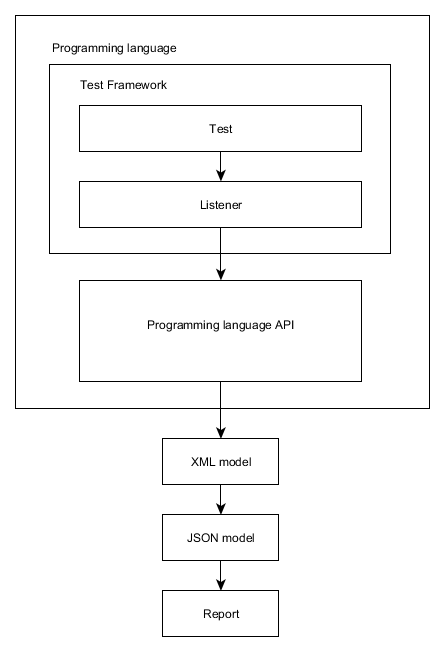
\includegraphics[height=160mm]{structure.png}
\caption{Общая схема фреймворка Allure}
\label{fig:allure}
\end{figure}

Используя свою реализацию RunListener можно построить собрать основную информацию о ходе выполнения теста. 

Подключение листенера, как правило, вынесено на уровень конфигурации запуска, что полностью удавлетворяет требованиям работы. Для адаптации тестового фреймворка достаточно реализовать листенер используя соответсвующее API языка программирования.

Однако стоит заметить, что не всю необходимую информацию о ходе теста можно собрать используя листенер, так как он оперирует терминологией xUnit. Сбор остальной информации о тестах, например информацию о пройденных шагах и сделанных аттачментах, будет реализован на уровне API языка программирования.

\subsection{Programming language API}

API для языка программирования представляет из себя набор обработчиков событий и сами события, используя которые можно полностью описать жизненный цикл теста. Программный интерфейс содержит в себе следующие события:

\begin{itemize}
\item начало/конец тестового запуска;
\item начало/конец тест суита;
\item начало/конец тест кейса;
\item начало/конец шага;
\item сохранение аттачмента;
\item добавление параметров запуска/тест суита/тест кейса;
\item изменение статуса теста/шага;
\item добавление пометок к тесту.
\end{itemize}

С использованием API для языка программирования сильно упрощается написание и поддержка листнеров для тестовых фреймворков. Вся собранная информация о ходе тестов сохраняется в XML модель. 

\subsection{XML model}

Собранная о тесте информация сериализуется в виде XML файлов. Для каждого теста создается свой файл. Сохраняются только те данные, которые нельзя синтезировать, что упрощает реализацию и поддержку интерфейса для языка программирования. Простейший пример сохранненной информации об одном тесте:

\begin{lstlisting}[style=XML, caption=Пример простой XML-модели]
<?xml version="1.0" encoding="UTF-8" standalone="yes"?>
<ns2:test-suite xmlns:ns2="urn:model.allure.qatools.yandex.ru" start="1400681607876" stop="1400681627123">
    <name>my.company.SampleTest</name>
    <test-cases>
        <test-case start="1400681608883" stop="1400681608891" status="passed">
            <name>test_pass</name>
        </test-case>
    </test-cases>
    <labels/>
</ns2:test-suite>
\end{lstlisting}

\subsection{JSON model}

На следующем этапе данные конвертируются в более удобный для отображения формат. Например, данные заранее группируются для различных отображений в отчете (xUnit, BDD, Defects). Также считается статистическая информация и генерируются данные для графиков.

Преборазование между моделями происходит с помощью XSLT. 

\subsection{Report}

Отображает результаты разными способами: 

\begin{itemize}
\item xUnit --- в данном табе используется терминология xUnit. Сначала тесты группируются по тест суитам, затем по самим тестам. Также присутствует возможность сортировать тесты по имени, важности, статусу и времени выполнения.
\item BDD --- данный таб используется для отображения результатов проверки требований к продукту. Сначала тесты группируются по требованию, потом по истории. Позволяет сразу понять, какие требования нарушаются в тестируемом продукте.
\item Defects --- группирует тесты по тексту сообщения. Также разбивает все ошибки на две группы --- продуктовые дефекты и ошибки тестов. 
\item Timeline --- отображает ход выполнения тестов с течением времени. Помогает находить ошибки типа "вчера в 15:30 сервис не работал".
\end{itemize}

Также есть различные графики, отображающие картину выполнения тестов в целом. Каждое из этих отображений результатов полезно разным людям. Менеджеру --- BDD, разработчику --- xUnit, тестировщику --- Defects. Отчет хорошо работает с большим количеством тестов (десятки тысяч).

\section{Сравнение}

Как было сказано ранее, на момент написания автором работы, систем, решающих поставленную задачу не было. Были рассмотрены системы, которые решали эту задачу частично. В данном разделе сравниваются эти системы с Allure Framework.


\begin{center}
\begin{tabular}{ | p{4cm} | p{4cm} | p{4cm} | p{4cm} | }
\hline
& Surefire & Thucydides & Allure Framework \\ \hline
Статус теста & Да & Да & Да \\ \hline
Сообщение об ошибке & Да & Да & Да \\ \hline
Длительность теста & Да & Да & Да \\ \hline
Сценарий теста & Нет & Да & Да \\ \hline
Возможность сохранения аттачментов & Нет & Только скриншоты & Да \\ \hline
Параметры теста & Нет & Нет & Да \\ \hline
Простое подключение & Да & Нет & Да \\ \hline
Типы тестов & В основном модульные & Тесты на веб-интерфейс с использованием WebDriver & Любые \\ \hline
BDD & Нет & Да & Да \\ \hline
Поддерживает основные языки программирования и тестовые фремворки & Да & Только JUnit (Java) & Да \\ \hline
\end{tabular}
\end{center}


